\section{DNA}


The idea of DNA as a personal \textit{blueprint} seems so obvious to us, but for the most
part of history the phenomenon of heredity was a big mystery. Greek thinkers like
Aristotle and Hippocrates spent years developing entire heredity theories to explain why
you look so much like your parents.

This astounding insight of Aristotle would go unnoticed until the late 20th century, but
in the end the ancient Greeks proved again how far ahead of their time they were. In 1869
Friedrich Meicher discovered a new microscopic substance in pus found on discarded
surgical bandages. He would call this substance "Nuclein" because it originated form the
nucleus of the cell. Yet another hundred years would pass until scientists proved that
this mysterious substance, now called "Deoxyribonucleic acid" or DNA, plays a central
role in heredity. In 1953 the last big question in the DNA mystery was resolved. Francis
Crick  and James Watson published what is now accepted as the first correct double-helix
model of the DNA structure.\\\\

Nowadays, it is well known that DNA exists out of two strands formed together to make a
double helix, shown in figure \ref{fig:DNA-model}. In this figure the major and minor
grooves of DNA are clearly portrayed. The DNA strands are a repetition of nucleotides,
composed of a sugar (deoxyribose), a phosphate group and just one of four nucleobases
[cytosine(C), guanine(G), adenine(A) or thymine(T)]. The two strands are connected
through these bases and only two combinations can occur: adenine and thymine, cytosine
and guanine. Technically DNA is a polynucleotide but it can also be seen as a polymer.
The big difference between an \textit{ordinary} polymer and DNA is that DNA has a more
diverse choice of bases (four), whereas \textit{ordinary} polymers repeat one and the
same monomer. The distance between two base-pairs for DNA is approximately 0.34 nm .\\

The double helix structure of DNA is observed in three different types:  the A-, B- and
Z-forms of DNA (figure \ref{fig:DNA-model2}). Both the A- and B-Form are right-handed
helices, while the Z-form is characterised by its left-handed helix. The A-from of DNA is
a compact helical structure resembling a double stranded RNA polymer and is often seen in
dehydrated DNA samples. The B-from is the most common form of DNA and the form we will
discuss in this project. The Z-form of DNA is mostly seen when there is a high torsional
strain on the helix or if DNA is in a solution with a high ionic concentration.

\begin{wrapfigure}{r}{0.23\textwidth}
  \begin{center}
    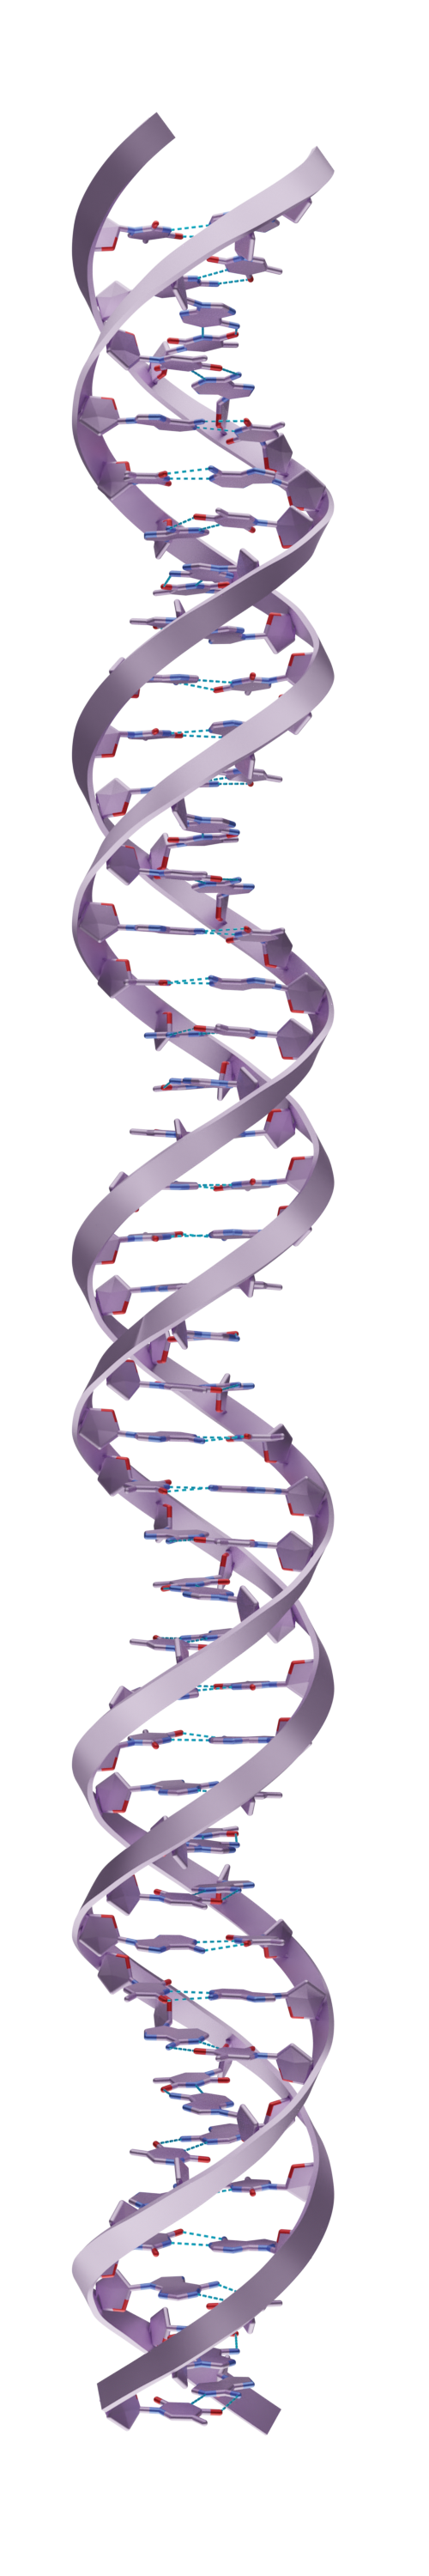
\includegraphics[width=0.20\textwidth]{Figures/DNA1.png}
  \end{center}
  \caption{;laskdjfal;s kjdf;a lskdfjl;askjdfl; askdfl;kasjdf w}
\end{wrapfigure}
